\subsection{Overview}

    \begin{figure}[H]
        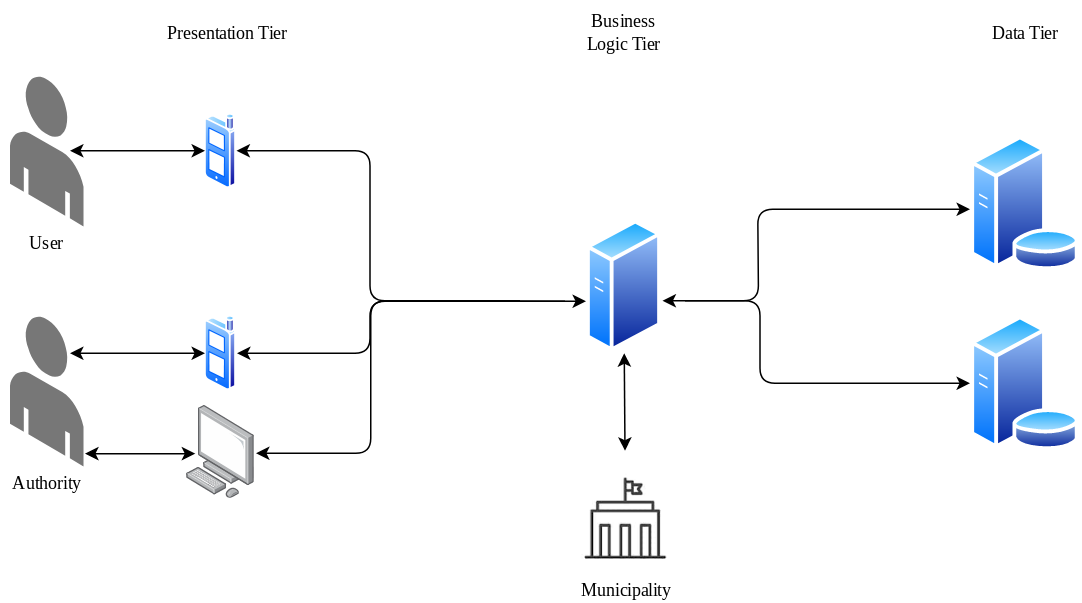
\includegraphics[width=\textwidth]{Images/SystemOverview.png}
        \caption{\label{fig:SystemOverview}High level overwiew of the system}
    \end{figure}

    The project is developed using a three-tier architecture implementation to properly separate the levels of Presentaion, Application and Data.
    The choice leads to the concept of "thin client": the client that has no knowledge of the logic behind the Application, but knows well how to interact with it 
    and exploit its services. This guarantees the App being "light" on resources and power consumption (the citizens do not need to have a high end smartphone).
    This leads to a high level of Mantainability and Scalability (a quality well appreciated to keep up with the expansion of the city).

\newpage

\subsection{Component view}

    \begin{figure}[H]
        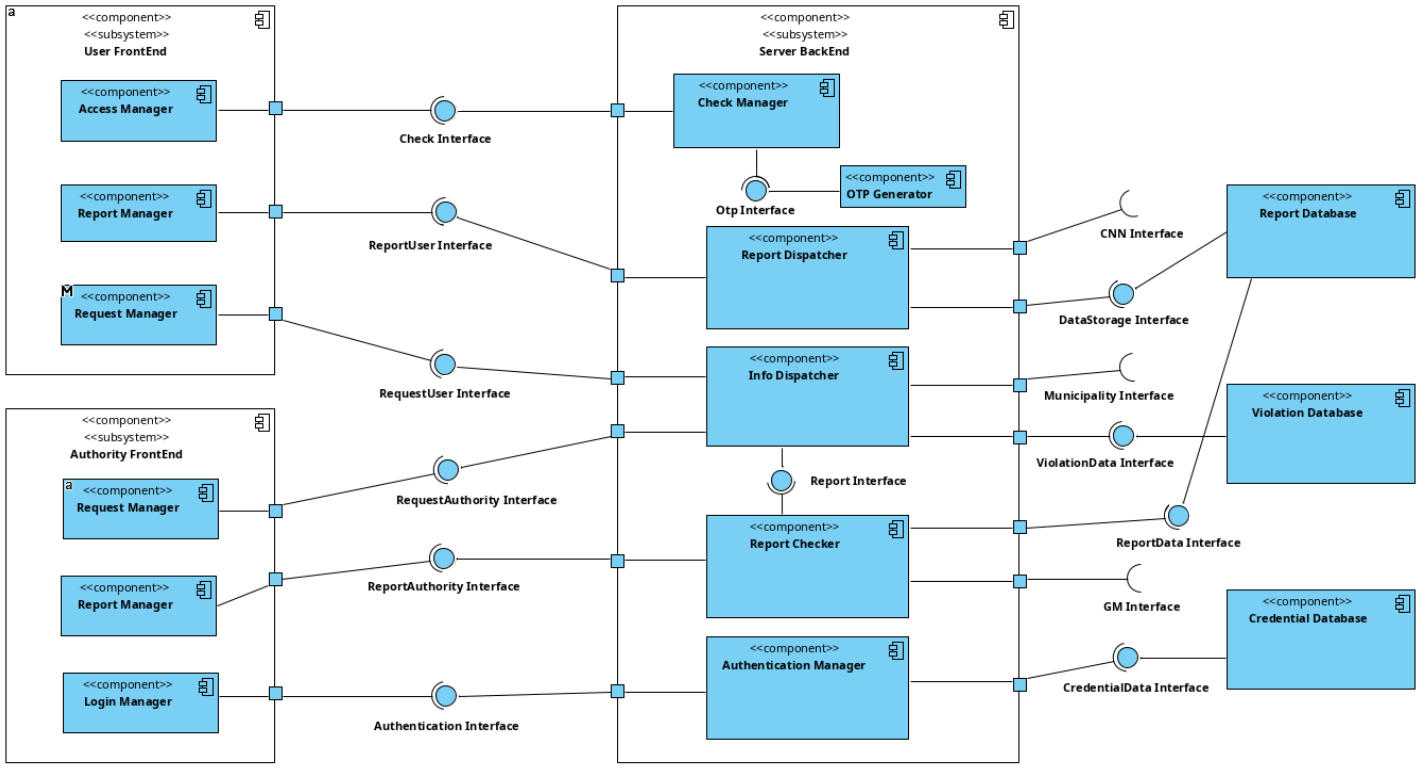
\includegraphics[width=\textwidth]{Images/ComponentView.png}
        \caption{\label{fig:ComponentView}Component diagram}
    \end{figure}

    The UML Component diagram shows the internal modular structure of the componentsand their connections. 
    To communicate, they can require a variable number of interfaces and attributes. 
    A brief description of each component, w.r.t the most importants interfaces, is presented:

    \begin{itemize}

        \item (Presentaion) Clients: Citizens' and authorities' machines, they can be either mobile devices or computers.
        
        \begin{itemize}

            \item Citizen Frontend

            \begin{itemize}

                \item Report Manager: Establishes an exchange of messages with the Server and sends data regarding the alleged violation, to be later examined.
                
                \item Request Manager: Retrieves the list of violations or accidents using the Server.
                
            \end{itemize}

            \item Authority Frontend

            \begin{itemize}

                \item Report Manager: Retrieves a report and orders to approve it or to discard it, based on the information stored.
                
                \item Request Manager: Retrieves the list of violations or accidents using the Server.
                
            \end{itemize}
            
        \end{itemize}

        \item (Application) Server Backend: Interacts with the clients and the Databases and contains the logic of the Application.
        
        \begin{itemize}
            \item Check Manager: Requests and receives the OTP by OTPGenerator to withstand the login of the citizen
            
            \item Report Dispatcher: Receives the information about the reports filed by citizens, completes them with data obtained by the CNN API 
                (a.k.a the recognized plates) and pushes them to the Report Server if the report is correctly fulfilled, aborting the incorrect ones.

            \item Authentication Manager: Exchanges information with the Database containing the credentials of the authority that wants to login
                and ultimates the login process
            
            \item Info Dispatcher: Communicates with both the types of users to retrieve information about violations or accidents (these are 
                retrieved by the Municipality API). \textit{Note: different kinds of users receive different quantities of information, for example, 
                citizens do no obtain the license plates of the offenders.}

            \item Report Checker: Sends information about the open reports to AuthorityFrontend::ReportManager, 
                locates the position using GM API and receives the approval of dismissal of said reports to store them as 
                Violations on the Violation Database or not, by sending them to InfoDispatcher.

        \end{itemize}
        
        \item (Data) Databases: Composed of three different elements (as different levels of security and replication are needed),
        they exchange messages with the Server, they allow the retrieval and addition of data.

        \begin{itemize}

            \item  Report Server: The data saved on this server is not important as reports are very dependent on time. The images and information
                stored are not legally binding (only authorities can administer fines), thus it must be able to handle large quantities of data and 
                be operative in a short span of time but data loss can be sustained.

            \item Violation Server: The data stored here is composed of light elements (only text) which do not require particular encryption thus the server 
                is able to sustain a great deal of ACID operations but requires data duplication.

            \item Credentials Server: This server contains information for the Authentication of the authorities so, not only does it require data duplication
                to be quickly operative also in case of failure, but encryption is also crucial to this device. Data is stored following good pratices of 
                security (e.g. only the salted hashes of the password are saved).     

        \end{itemize}
        
    \end{itemize}

\newpage



\subsection{Deployment view}

    \begin{figure}[H]

        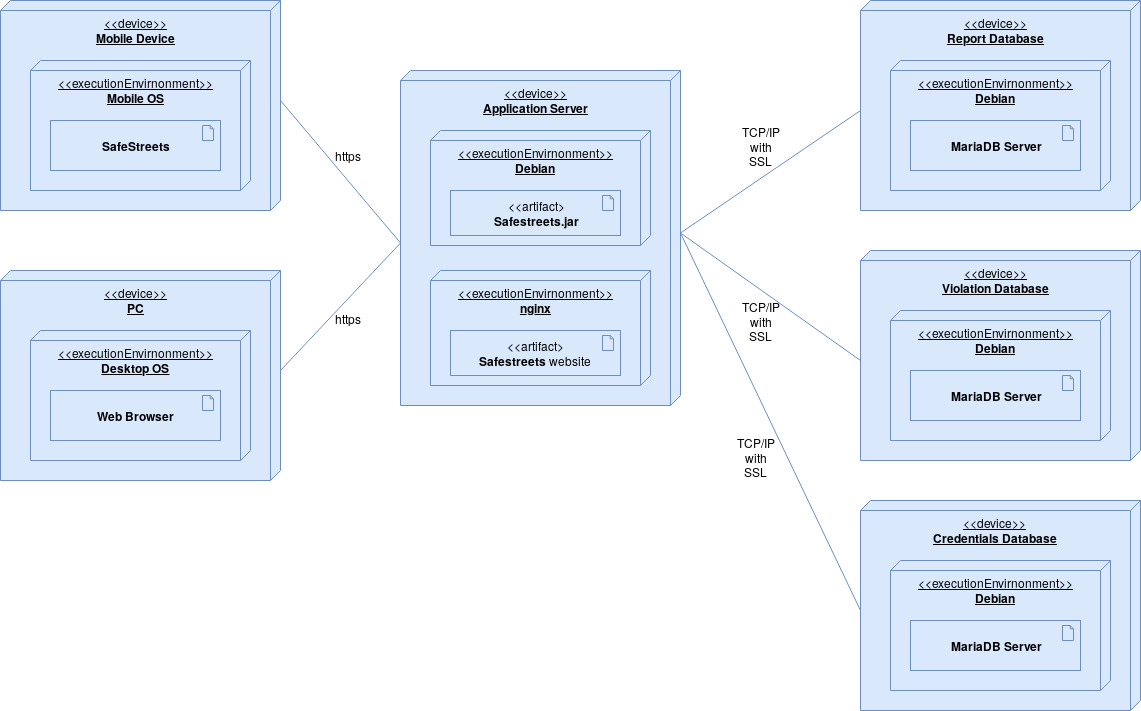
\includegraphics[width=\textwidth]{Images/deployment.jpg}
        \caption{\label{fig:deployment}Deployment diagram}
        
    \end{figure}
	
	The purpose of the Deployment diagram is to specify the distribution of the components of the system, showing the configuration of run time processing nodes and components that live on them. 

\newpage

\subsection{Runtime view}
\subsubsection{User Access}
	\begin{figure}[H]
		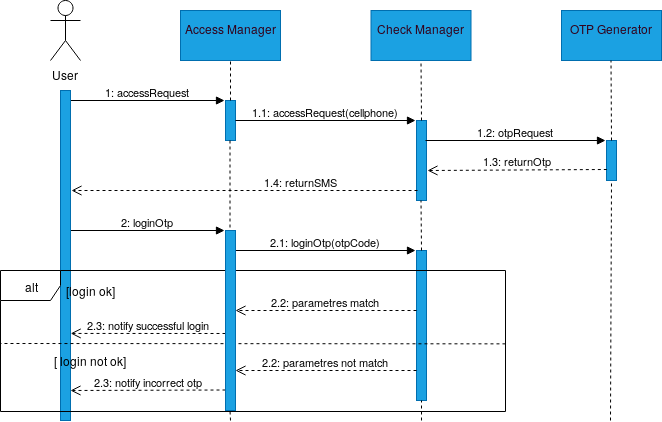
\includegraphics[width=\textwidth]{Images/RunTimeViewUserAccess.png}		
		\caption{\label{fig:UserAccess}User access sequence diagram}
	\end{figure}
\subsubsection{Authority Access}
	\begin{figure}[H]
		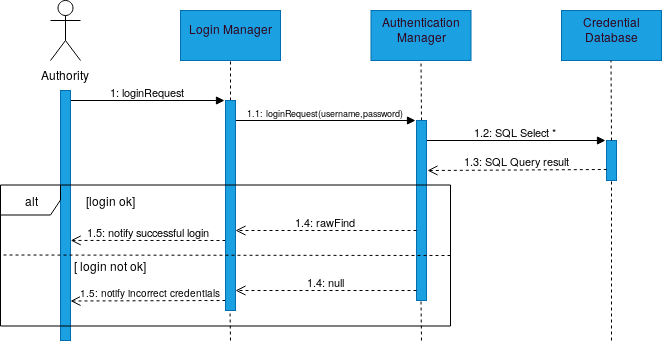
\includegraphics[width=\textwidth]{Images/RunTimeViewAuthorityAccess.png}
		\caption{\label{fig:AuthorityAccess}Authority access sequence diagram}	
	\end{figure}
\subsection{Component interfaces}

\subsection{Selected architectural styles and patterns}